\documentclass[10pt]{book}
\usepackage{gvv-book}
\usepackage{gvv}
\usepackage{float}
\usepackage[sectionbib,authoryear]{natbib}% for name-date citation comment the below line
\usepackage{setspace}
\setstretch{1.0}
%\usepackage[sectionbib,numbers]{natbib}% for numbered citation comment the above line
%%********************************************************************%%
%%       How many levels of section head would you like numbered?     %%
%% 0= no section numbers, 1= section, 2= section, 3= subsection %%
\setcounter{secnumdepth}{3}
%%********************************************************************%%
%%**********************************************************************%%
%%     How many levels of section head would you like to appear in the  %%
%%				Table of Contents?			%%
%% 0= chapter, 1= section, 2= section, 3= subsection titles.	%%
\setcounter{tocdepth}{2}
%%**********************************************************************%%
%\includeonly{ch01}
\makeindex
\let\cleardoublepage\clearpage
\begin{document}
\frontmatter
%%%%%%%%%%%%%%%%%%%%%%%%%%%%%%%%%%%%%%%%%%%%%%%%%%%%%%%%%%%%%%%%
\booktitle{Geometry}
\subtitle{Through Algebra}
\AuAff{Errala Paulsonashish}
%\halftitlepage
\titlepage
\tableofcontents
%\listoffigures %optional
%\listoftables  %optional
%% or Contributor Page for edited books
%% before \tableofcontents
%%%%%%%%%%%%%%%%%%%%%%%%%%%%%%%%%%%%%%%%%%%%%%%%%%%%%%%%%%%%%%%%
\setcounter{page}{0}
\begin{introduction}
This book shows how to solve problems in geometry using trigonometry and coordinate geometry. 
\end{introduction}
\mainmatter
\chapter{Triangle}
Consider a triangle with vertices
		\begin{align}
			\label{eq:tri-pts}
			\vec{A} = \myvec{-5 \\ -4},\,
			\vec{B} = \myvec{3 \\ -3},\,
			\vec{C} = \myvec{4 \\ 0}
		\end{align}
\section{Altitude}
\begin{enumerate}[label=\thesection.\arabic*.,ref=\thesection.\theenumi]
\numberwithin{equation}{enumi}

%Question 1.3.1: 
\item $\vec{D}_1$ is a point on $\vec{BC}$ such that
		\begin{align}
			\vec{AD_1} \perp \vec{BC}
		\end{align}
		and $\vec{AD_1}$ is defined to be the altitude. 
		Find the normal vector of $\vec{AD_1}$.\\
\solution\\
Given,
\begin{align}
\vec{A} = \myvec{-5 \\ -4},\\
\vec{B} = \myvec{3 \\ -3},\\
\vec{C} = \myvec{4  \\ 0}
\end{align}
Normal vector of $\vec{AD_1}$ is orthogonal to $\vec{AD_1}$ and hence parallel to $\vec{BC}$. Direction vector $\vec{m_{BC}}$\\
\begin{align}
	&= \vec{C} - \vec{B}\\
        &= \myvec{4 \\ 0} - \myvec{3 \\ -3}\\
        &= \myvec{1 \\ 3}\\
        \text{Normal vector of } \vec{AD_1} &= \myvec{ 1 \\ 3}
\end{align}

%Question 1.3.2:
\item Find the equation of $\vec{AD_1}$. \\
\solution\\
The normal vector of $\vec{AD_1}$ is
\begin{align}
\implies \vec{n} &= \myvec{1 \\ 3}
\end{align}
The equation of $\vec{AD_1}$ is
\begin{align}
 \vec{n}^{\top}(\vec{x-A}) &= 0 \\
 \vec{n}^{\top}(\vec{x}) &= \vec{n}^{\top}(\vec{A})\\
\implies \myvec{1 & 3}\vec{x} &= \myvec{1 & 3}\myvec{-5 \\ -4}\\
\myvec{1 & 3}\vec{x} &= -17
\end{align}

\begin{figure}[H]
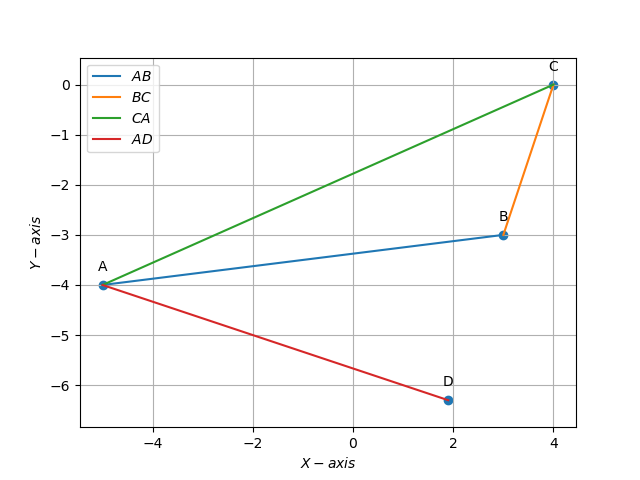
\includegraphics[width=\columnwidth]{figs/AD1_altitude.png}
\caption{Altitude $\vec{AD_1}$}
\label{fig:Altitude_AD1}
\end{figure}

%Question 1.3.3:
\item Find the equations of the altitudes $\vec{BE_1}$ and $\vec{CF_1}$ to the sides $\vec{AC}$ and $\vec{AB}$ respectively.\\
\solution\\
The normal equation of $\vec{BE_1}$ is 
\begin{align}
\vec{n} &= \myvec{9 \\ 4}\\
\vec{n}^{\top}\brak{\vec{x} - \vec{B}} & = 0 \\
\vec{n}^{\top} \brak{\vec{x}} & = \vec{n}^{\top} \brak {\vec{B}} \\
	\implies \myvec{9 & 4 }\vec{x} & = \myvec{9 & 4} \myvec{3 \\ -3}\\
	\implies \myvec{9 & 4}\vec{x} & = 15
\end{align}
The normal equation of $\vec{CF_1}$ is 
\begin{align}
\vec{n} &= \myvec{8 \\ 1} \\
\vec{n}^{\top}\brak{\vec{x}-\vec{C}} &= 0\\
\vec{n}^{\top}\brak{\vec{x}} &= \vec{n}^{\top}\brak {\vec{C}} \\
\implies \myvec{8 & 1}{\vec{x}} &= \myvec{8 & 1} \myvec{4 \\ 0}  \\
	\implies \myvec{8 & 1}\vec{x} &= 32
\end{align}
\begin{figure}[H]
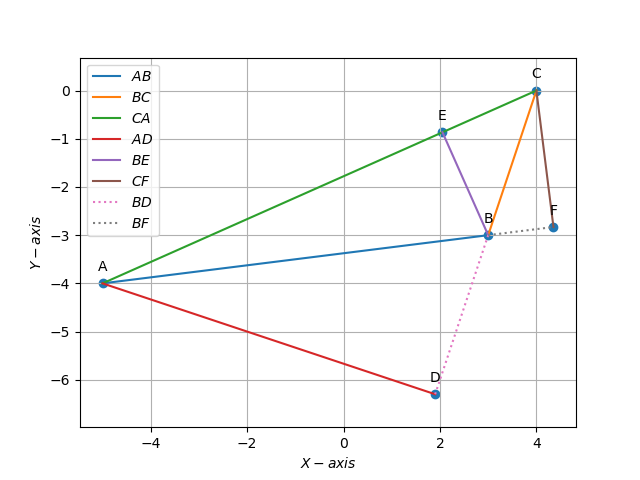
\includegraphics[width=\columnwidth]{figs/BECF_altitudes.png}
\caption{Altitudes $\vec{BE_1}$ and $\vec{CF_1}$ }
\label{fig:Line BE and CF}
\end{figure}

%Question 1.3.4:
\item Find the intersection $\vec{H}$ of $\vec{BE_1}$ and $\vec{CF_1}$.\\
\solution\\
 Equation of $\vec{BE_1}$ :
 \begin{align}
     \myvec{9 & 4}\vec{x} &= 15
 \end{align}
  Equation of $\vec{CF_1}$ :
 \begin{align}
    \myvec{8 & 1}\vec{x} &= 32
 \end{align}
Therefore, we need to solve the following equation to get $\vec{H}$ :
\begin{align}
        \myvec{9 & 4\\8 & 1} \vec{x} &= \myvec{15 \\ 32}
\end{align}
Solving the above equation by Gauss-Jordan method
\begin{align}
        \myvec{9 & 4 & 15 \\ 8 & 1 & 32}
	 \xleftrightarrow[]{R_1 \leftarrow \frac{R_1}{9}}
        \myvec{1 & \frac{4}{9} & \frac{5}{3}\\8 & 1 & 32}\\
	 \xleftrightarrow[]{R_2 \leftarrow R_2 - 8R_1}
        \myvec{1 & \frac{4}{9} & \frac{5}{3}\\0 & \frac{-23}{9} & \frac{56}{3}}\\
	 \xleftrightarrow[]{R_2 \leftarrow \frac{-9R_2}{23}}
        \myvec{1 & \frac{4}{9} & \frac{5}{3}\\0 & 1 & \frac{-168}{23}}\\
        	 \xleftrightarrow[]{R_1 \leftarrow R_1 - \frac{4R_2}{9}}
                  \myvec{1 & 0 & \frac{113}{23}\\0 & 1 & \frac{-168}{23}}
\end{align}
Therefore point of intersection $\vec{H}$ is
\begin{align}
	&= \frac{1}{23}\myvec{113 \\ -168}
\end{align}
\begin{figure}[H]
	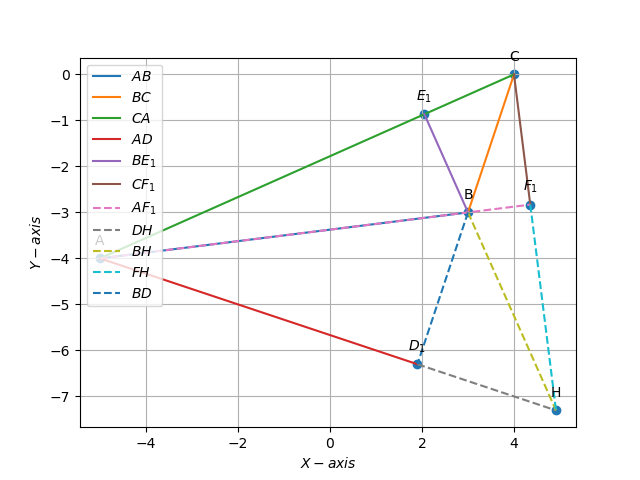
\includegraphics[width=\columnwidth]{figs/H_intersection.png}
	\caption{Intersection point $\vec{H}$ of altitudes $BE_1$ and $CF_1$}
\label{fig:Interction point}
\end{figure}

%Question 1.3.5:
\item Verify that 
		\begin{align}
			\brak{\vec{A}-\vec{H}}^{\top}\brak{\vec{B}-\vec{C}} = 0
		\end{align}\\
  \solution\\
Given,
\begin{align}
            \vec{A} = \myvec{-5 \\ -4},\\ 
            \vec{B} = \myvec{3 \\ -3}.\\
            \vec{C} = \myvec{4 \\ 0},\\
            \vec{H} = \frac{1}{23}\myvec{113 \\ -168}
\end{align}
To solve the equation
\begin{align}
\vec{A}-\vec{H} &= \myvec{-5 \\ -4} - \frac{1}{23}\myvec{113 \\ -168}\\
                &= \frac{1}{23}\myvec{-228 \\ 76}\\
\vec{B}-\vec{C} &= \myvec{3 \\ -3} - \myvec{4 \\ 0}\\
                &= \myvec{-1 \\ -3}\\
	\implies \brak{\vec{A}-\vec{H}}^{\top}\brak{\vec{B}-\vec{C}} &= \frac{1}{23}\myvec{-228 & 76} \myvec{-1 \\ -3}\\
                &= 0
\end{align}
\begin{figure}[H]
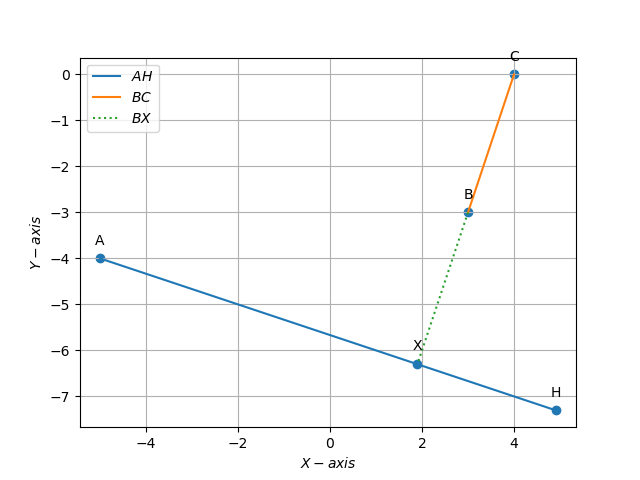
\includegraphics[width=\columnwidth]{figs/AHBC_verify.png }
\caption{Plot of points $A, B, C$ and $H$}
\label{fig1:Points}
\end{figure}

All cosdes for this section are available at
\begin{lstlisting}
	geometry/Triangle/Altitude/codes/All_Altitudes.py
\end{lstlisting}
\end{enumerate}
\backmatter
\appendix
\latexprintindex
\end{document}
